\documentclass[11pt,a4paper]{article}

\input{packages.tex}
\input{commands.tex}

\usepackage[utf8]{inputenc}
\usepackage[T1]{fontenc}
\usepackage[english]{babel}
\usepackage{lmodern}

\linespread{1.2}
\usepackage{geometry}
\geometry{
	left=2.65cm,
	right=2.65cm,
	top=3.2cm,
	bottom=3.2cm,
	marginparwidth=2cm,
}

\usepackage{scrlayer-scrpage}
\pagestyle{scrheadings}
\clearpairofpagestyles

\chead{\headmark}
\automark[section]{section}
\automark*[subsection]{}
\cfoot*{\pagemark} 

\usepackage[backend=biber, sorting=nyt, maxbibnames=99]{biblatex}
\usepackage{csquotes}
% \addbibresource{literature.bib}

\usepackage{url}

\usepackage{mathtools}
\usepackage{amssymb}
\usepackage{amsthm}
\usepackage{wasysym}
\usepackage{latexsym}

\usepackage{setspace}

\usepackage{nicefrac} 

\usepackage{relsize} 

\usepackage{extarrows}
\usepackage{stmaryrd} 

\usepackage[new]{old-arrows}

\usepackage{accents} 

\usepackage{graphicx}
\usepackage{float}
\usepackage{floatflt}
\usepackage{rotating}
\usepackage{color}
\usepackage[absolute]{textpos}

\usepackage{here}

\usepackage{epic}
\usepackage[percent]{overpic}
\usepackage{caption}
\usepackage{subcaption}
\usepackage{capt-of}

\usepackage{tikz}
\usetikzlibrary{matrix}
\usetikzlibrary{cd}

\usepackage{xcolor}
\definecolor{green-new}{rgb}{0.0,0.5,0.0}

\usepackage{multirow}

\usepackage{chngcntr}
\counterwithin{figure}{section}
\counterwithin{table}{section}

\usepackage{comment} 

\hypersetup{
	colorlinks	= true, 
	linkcolor	= green-new,
	urlcolor	= blue,
	citecolor	= blue
}

\usepackage{cleveref}

\usepackage{thmtools}

\crefformat{footnote}{#2\footnotemark[#1]#3} 

\counterwithout{figure}{section}

\newcommand{\tagaligneqn}{\refstepcounter{equation}\tag{\theequation}} 

\newcommand{\cC}{\mathcal{C}}
\newcommand{\cF}{\mathcal{F}}
\newcommand{\cM}{\mathcal{M}}
\newcommand{\cP}{\mathcal{P}}
\newcommand{\cQ}{\mathcal{Q}}
\newcommand{\cV}{\mathcal{V}}

\newcommand{\sC}{\textsf{C}}

\newcommand{\wt}[1]{\widetilde{#1}}
\newcommand{\wtr}[1]{\widetilde{#1\,}\!} 

\newcommand{\co}{\colon\thinspace}
\newcommand{\comp}{\mathbin{\circ}} 

\newcommand{\abs}[1]{\left\lvert #1 \right\rvert}
\newcommand{\norm}[1]{\left\lVert #1 \right\rVert} 

\newcommand{\pr}[1]{\textsf{pr}_{#1}} 

\makeatletter
\newcommand*\bigcdot{\mathpalette\bigcdot@{.5}}
\newcommand*\bigcdot@[2]{\mathbin{\vcenter{\hbox{\scalebox{#2}{$\m@th#1\bullet$}}}}}
\makeatother

\newcommand{\Ob}{\textsf{Ob}}



\newcommand{\op}{\textup{op}}

\newcommand{\tcolor}[1]{\textcolor{red}{#1}}
\newcommand{\red}[1]{\textcolor{red}{#1}}
\newcommand{\gray}[1]{\textcolor{gray}{#1}}

\DeclareMathOperator*{\colim}{colim}

\setlength\emergencystretch{1em}

\numberwithin{equation}{section}

\theoremstyle{definition}
\newtheorem*{defi}{Definition}
\newtheorem*{rmk}{Remark}
\newtheorem*{eg}{Example}
\newtheorem*{constr}{Construction}

\theoremstyle{plain}
\newtheorem*{thm}{Theorem}
\newtheorem*{prop}{Proposition}

\allowdisplaybreaks[1]



\addbibresource{literatureHtpyThryOfGraphs.bib}

\title{Homotopy Theory of Graphs}
\author{Jana Nickel \& Markus K. Youssef}
\date{}

\begin{document}


\maketitle

\section{Some Preliminary Thoughts}
\subsection{Homotopy Theory}
\begin{flushright}
  \emph{“It is an unfortunate coincidence that homotopy theory originated in the theory of spaces.”}\\
  — a friend (permission to quote pending). 
\end{flushright}
Homotopy theory can be seen as \say{the study of sameness}. Quite early in mathematics one is confronted with the idea that \say{equality}, taken literally, is too strict of a notion to compare mathematical objects with each other. In practice, we are more interested in how an object \emph{behaves} rather than how it is explicitly constructed. This idea is formalized by the notion of \emph{isomorphism}: two objects are isomorphic when they cannot be told apart for the purposes at hand.
\begin{example}
    Take the \href{https://ncatlab.org/nlab/show/walking+structur}{walking edge} $K_2$, i.e., \say{the} graph with two vertices joined by a single edge. It admits countless concrete representations, but what we really mean by $K_2$ is the \say{idea} of this graph, more than how it is constructed. One can choose the vertex set to be $\{0, 1 \}$, or $\{\texttt{red}, \texttt{blue}\}$, or even $V(K_2) = \{\R, + \}$; as long as exactly one edge connects the two vertices, any such realization can rightfully be called \emph{the} graph $K_2$.
\end{example}
Two objects are isomorphic, if there exists \emph{some} isomorphism between them. Sometimes, however, we would like to keep track of \emph{how} we identified these two objects.\\
Coming back to the example above, there are exactly two isomorphisms from (any) $K_2$ to (any other) $K_2$. So, instead of simply saying two objects are isomorphic, we now get an entire \say{set of isomorphisms} telling us precisely in which way these two objects are being identified. \\
Taking this one step further, we note that inside an ordinary set, the only way we can compare two elements is via (strict) equality: two elements are either equal or not. We can now ask the question: What if the set of isomorphisms itself carries some additional structure, allowing us to talk about \say{isomorphisms of isomorphisms}? \\
Suppose, for example, that every hom-set $\Hom(X, Y)$, is not merely a set, but carries an extra structure -- say, an equivalence relation.\footnote{Note that general model categories do not require the existence of such an equivalence relation, whereas the approach with higher categories taken below, requires an even richer structure on $\Hom$ than just an equivalence relation.}\\
This new notion of sameness between morphisms is called a \emph{homotopy} and we write $f \simeq g$ when $f$ and $g$ lie in the same equivalence class (in practice, we would call a homotopy a concrete \say{witness} of this identification). We now would want to understand how this relaxed notion of sameness between maps trickles down to the original objects we wanted to study.
\begin{example}
    Let us consider what happens if we identify \emph{all} ways of comparing an object to itself, i.e. if every endomorphism is considered to be homotopic to the identity. Take $K_2$ and the $4$-cycle graph $C_4$ and pick two maps
    \[
        f\colon K_2 \longrightarrow C_4,
        \qquad
        g\colon C_4 \longrightarrow K_2.
    \]
    Now, the two compositions of these maps are  homotopic to the identity, i.e. $g \circ f \simeq \id_{K_2}$ and $f \circ g \simeq \id_{C_4}$. In other words, even though neither $f$ nor $g$ is an isomorphisms, they are, in a certain sense, \emph{inverses} of each other. \\
    There is a new way in which we can say that $K_2$ and $C_4$ are the same object: we say that $K_2$ and $C_4$ are \emph{homotopy equivalent}.
\end{example}
In summary, we can organize our various notions of sameness into the following hierarchy: 
\begin{itemize}
    \item \textbf{Equality}: two objects are (strictly) \emph{equal} when they literally coincide, That is, no maps between them are considered.
    \item \textbf{Isomorphism}: two objects are \emph{isomorphic} if there are morphisms $f,g$ with $g\!\circ\!f=\id$ and $f\!\circ\!g=\id$. That is, if there exists a pair of inverse maps, and maps are compared by (strict) equality.
    \item \textbf{Homotopy equivalence}: two objects are homotopy equivalent when there are morphisms $f,g$ with $g \circ f\simeq\id$ and $f \circ g\simeq\id$. That is, if there exists a pair of inverse maps, and maps are compared by homotopy.
\end{itemize}
Homotopy theory, in the broadest sense, is the machinery that tracks these ever more sublte layers of sameness. In what follows, we will encode this hierarchy in the language of higher categories. While, in principle, nothing is stopping us from talking about \say{homotopies of homotopies of homotopies (and beyond)}, we will only take the first step on this ladder and sketch how the pattern extends to the general setting.

\subsection{Higher Categories}
\begin{flushright}
  \emph{“Higher categories are like a category, but iwth morphisms between morphisms (and so on, ad infinitum), all stacked like an infinitely tall, anxiety-inducing layer cake of abstraction.”}\\
  — another friend (permission to quote pending). 
\end{flushright}
Category theory compels us to compare objects without ever \say{opening them up.}  
Instead of peering inside an object, we study the web of morphisms that ties it to every other object. Two objects therefore count as \emph{the same} when, in the language internal of the category itself, we cannot tell them apart -- that is, when they are isomorphic. \\

In the usual (locally small) setting of a category $\Ccal$ each Hom-collection $\hom_{\Ccal}(c,d)$ is merely a \emph{set}, so different morphisms can be compared only by strict equality.  If we want a softer notion of sameness \emph{between morphisms}, the natural move is to let the Hom-set carry more
structure; namely, the structure of a \emph{category}.  Concretely, fix two objects $c,d \in \Ccal$; now regard the morphisms $f,g \colon c \to d$ as
\emph{objects} of a new category and introduce \say{morphisms between morphisms} $\alpha \colon f \Rightarrow g$. To keep track of the levels we adopt the standard terminology:

\begin{itemize}
  \item $0$-cells: the original objects $c,d$;
  \item $1$-cells: the morphisms $f,g\colon c \to d$;
  \item $2$-cells: the homotopies $\alpha \colon f \Rightarrow g$.
\end{itemize}

Equipping every Hom-set with this internal structure and adding some coherence axioms gives exactly a \emph{$2$-category}.  Once we have $2$-cells we can again pass to a coarser view by declaring two $1$-cells equivalent when they are connected by a $2$-cell.  Collapsing in this way
produces the \emph{homotopy category} $\mathrm{ho}\Ccal$: it keeps the original objects but replaces each Hom-set by the set of equivalence classes of $1$-cells. \\

Nothing stops us from iterating.  If each Hom-category is itself a $2$-category, then $\Ccal$ becomes a $3$-category; collapsing $3$-cells yields a $2$-category, and collapsing once more returns us to an ordinary category. This two-step \say{collapse procedure} is precisely how the authors of the paper discussed below build their homotopy category: they first extract a $2$-category from (the shadow of) a $3$-category, and then collapse it further to obtain the desired homotopy category.

\newpage

\section{Homotopy Theory of Grpahs}

Homotopy theory originated in the context of topological spaces. In classical homotopy theory, one considers continuous transformations of topological spaces and continuous maps between them.
There are various approaches to study the notion of homotopy in categories of graphs. Since graphs form discrete mathematical structures, it is not immediately clear how to translate the continuous concept of homotopy into the setting of graphs. 
The probably first approach to develop a homotopy theory of graphs was the construction of a certain polyhedral complex, called \textit{Hom complex}, which encodes information about the morphisms between two graphs. It was then endowed with a topology so that one can study its homotopy. This approach is treated for example in \cite{Babson-et-al, Babson-Kozlov, Fieux-Lacaze, Kozlov_Chromatic, Kozlov_A-simple-proof, Kozlov_Collapsing, Kozlov_Simple-htpy}.
Another way was more recently suggested by A.~Dochtermann, who introduced the notion of $\times$-homotopy for graphs (pronounced ``cross homotopy''), using only category theoretical constructions within the category of graphs, see~\cite{Dochtermann_Hom-complexes}. It turned out that this gives rise to the same homotopy theory as the one resulting from simplicial techniques. Since then, there has been many results following this approach, as exemplified in \cite{Dochtermann_Homotopy, Chih-Scull, Droz, Goyal-Santhanam, Plessas}. 
	%
Our blog post is based on T.~Chih and L.~Scull's paper~\cite{Chih-Scull}. In particular, we will follow this second approach, allowing us to study homotopy theory of graphs by means of explicit discrete constructions.
Besides, all figures are taken from this reference.

\section*{A 2-category of graphs}	
	
	The definition of a graph is not consistent in literature. In fact, there are many different definitions, depending on various properties, such as the existence of loops and multiple edges, for instance. For us, a \textit{graph} will mean an undirected (perhaps infinite) pseudograph without multiple edges. More precisely, a \textit{graph} is a pair $G=(V(G),E(G))$ consisting of a set $V(G)$ of \textit{vertices} and a set $E(G)$ of \textit{edges}, which are sets of one or two vertices $v,w$ and denoted as $v\sim w\in E(G)$, or simply, $v\sim w$. If $v\sim v\in E(G)$, we say that $v$ is a \textit{looped vertex}. 
	
	Graphs are the objects of a category $\Grph$ whose arrows are \textit{graph morphisms}. Since our graphs are not allowed to contain multiple edges, a graph morphism is uniquely determined by its action on vertices. Explicitly, a \textit{morphism} $f\co G\to H$ \textit{of graphs} is a map $f\co V(G)\to V(H)$ of vertex sets which preserves adjacency, in the sense that $v\sim w\in E(G)$ implies $f(v)\sim f(w)\in E(H)$.
	
	\bigskip
	We want to study homotopy theory in the category $\Grph$ of graphs, following the procedure in~\cite{Chih-Scull}. In particular, we will work with the notion of $\times$-homotopy, which is quite similar to the classical homotopy of topological spaces. However, we will need a substitute for the closed real unit interval $[0,1]$, which is essential for the definition of a continuous homotopy of spaces. Again, there are various possibilities to replace the interval $[0,1]$ when studying homotopies of graphs. We will choose looped path graphs as defined further below.
	Another important ingredient for a continuous homotopy is the product of two topological spaces. Our category~$\Grph$, as well, admits a categorical product, which is defined as you might expect:
	
	\begin{defi}
		Given a pair of graphs $G$ and~$H$, their \textit{product graph} $G\times H$ is defined by 
		\begin{align*}
			V(G\times H) &\coloneqq V(G)\times V(H), \\
			E(G\times H) &\coloneqq \{ (v_1,v_2)\sim (w_1,w_2)\mathbin| v_1\sim w_1\in E(G), v_2\sim w_2\in E(H) \}.			
		\end{align*}
	\end{defi}

	\noindent Figure~\ref{fig:product-graph} shows an example of a product graph.
	
	\begin{figure}[H]
		\centering
		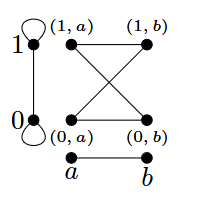
\includegraphics[width=0.25\textwidth]{figures/product-graph}
		\caption{Example of a product graph.}
		\label{fig:product-graph}
	\end{figure}
	
	Recall that for ``nice'' topological spaces, the product functor $X\times(-)$ admits a right adjoint, given by the exponential. The same is true in our category of graphs, yielding the notion of the exponential graph $H^G$. Yet, its definition seems a bit curious at first glance because its vertex set comprises all maps of sets from $V(G)$ to~$V(H)$ and not only the graph morphisms from $G$ to~$H$. Nevertheless, from a category theoretical perspective, this phenomenon does not seem that strange. In fact, working for example in the category of directed pseudographs, aka quivers, defined as presheaves on the category $V\rightrightarrows E$, the vertex set of the exponential takes the same form.
	
	\begin{defi}
		The \textit{exponential graph} $H^G$ is defined by
		\begin{align*}
			V(H^G) &\coloneqq \{ \textup{set maps } f\co V(G)\to V(H) \}, \\
			E(H^G) &\coloneqq \{ f\sim g\mathbin| \forall v\sim w\in E(G): f(v)\sim g(w)\in E(H) \}.
		\end{align*}
	\end{defi}
	
	Although the vertex set of the exponential does not capture the graph morphisms, we can recover the graph morphisms by the looped vertices. Indeed, note that a looped vertex of~$H^G$ is precisely a graph morphism $G\to H$.
	Figure~\ref{fig:exponential-graph} illustrates an example of an exponential graph, where a vertex $f\in V(H^G)$ is written as a pair $(f(0),f(1))$.
	
	\begin{figure}[H]
		\centering
		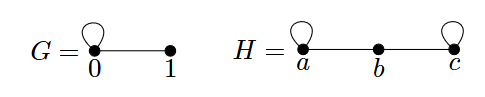
\includegraphics[width=0.5\textwidth]{figures/exponential-graph-input}
	\end{figure}	
	\vspace{-0.5cm}
	\begin{figure}[H]
		\centering
		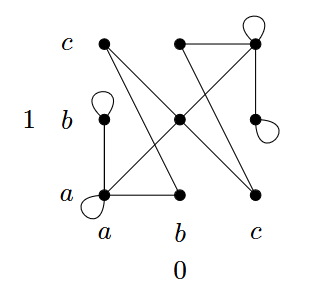
\includegraphics[width=0.35\textwidth]{figures/exponential-graph-output}
		\caption{Example of an exponential graph.}
		\label{fig:exponential-graph}
	\end{figure}
	
	As promised, there is the following result:
	
	\begin{prop}
		For every graph $G$, the product functor $G\times(-)\co\Grph\to\Grph$ is left-adjoint to $(-)^G\co\Grph\to\Grph$,
		\begin{equation*}
			\begin{tikzcd}
				\Grph
				\arrow[bend left = 50]{r}{G\times (-)}
				\arrow[r, phantom, "\raisebox{-0.2ex}{\rotatebox{270}{$\dashv$}}"]
				& \Grph.
				\arrow[bend left = 50]{l}{(-)^G}
			\end{tikzcd}
		\end{equation*}
		
		\bigskip
		In particular, for any three graphs $G,H,J$, there is a bijection
		\[ \Grph(G\times H, J) \cong \Grph(H, J^G). \]
	\end{prop}
	
	We will now define path graphs and their looped version.
	
	\begin{defi}
		The \textit{path graph of length~$n$} is the graph $P^n$ whose vertex set is $V(P^n)\coloneqq \{ 0,1,\dots,n \}$ and whose edge set is $E(P^n)\coloneqq \{ i-1\sim i\mathbin| i\in \{ 1,\dots,n \} \}$.
		Turning every vertex into a looped vertex, we obtain the \textit{looped path graph $I^n_\ell$ of length~$n$}.
		
		\begin{figure}[H]
			\centering
			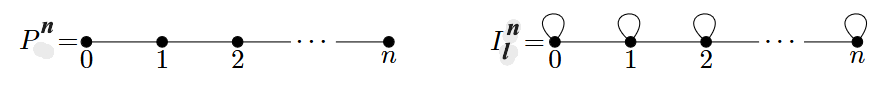
\includegraphics[width=0.8\textwidth]{figures/path-graph-looped-path-graph-bearbeitet}
		\end{figure}
	\end{defi}
	
	Using these path graphs, we can now consider walks and looped walks in a graph, which constitute a discrete analogue of continuous paths in a topological space.

	\begin{defi}
		A \textit{walk} in a graph~$G$ \textit{of length~$n$} is a graph morphism $\alpha\co P^n\to G$.
		Similarly, we define a \textit{looped walk} in~$G$ \textit{of length~$n$} to be a graph morphism $\alpha\co I^n_\ell\to G$.
		If $\alpha(0)=x$ and $\alpha(n)=y$, we say that $\alpha$ is a (looped) walk \textit{from $x$ to~$y$}.
	\end{defi}	
	
	Observe that we can think of a walk $\alpha\co P^n\to G$ as a sequence $(\alpha(0),\dots,\alpha(n))$ of vertices $\alpha(i)\in V(G)$ with the property that any two consecutive vertices are adjacent: $\alpha(i-1)\sim\alpha(i)\in E(G)$ for all $i\in \{1,\dots,n \}$.
	A looped walk $\alpha\co I^n_\ell\to G$ can be analogously viewed as a sequence $(\alpha(0),\dots,\alpha(n))$ of \textbf{looped} vertices $\alpha(i)\in V(G)$ with $\alpha(i-1)\sim\alpha(i)\in E(G)$ for all $i\in \{1,\dots,n \}$.

	By virtue of our aim to study $\times$-homotopy of graphs, we will be mainly interested in looped walks, so let us restrict to those. But be aware that the following concepts can be also applied to walks.
	
	\begin{defi}
		Let $\alpha\co I^n_\ell\to G$ be a looped walk from $x$ to $y$, and let $\beta\co I^m_\ell\to G$ be a looped walk from $y$ to $z$. Their \textit{concatenation} is the looped walk
		\[ \alpha\bigcdot\beta\co I^{n+m}_\ell\to G \]
		where
		\[ (\alpha\bigcdot\beta)(i)\coloneqq \begin{cases}
			\alpha(i) & i\in\{0,\dots,n\} \\
			\beta(i-n) & i\in\{n,\dots,n+m\}.
		\end{cases} \]
	\end{defi}

	\medskip
	\noindent This definition is visualized in Figure~\ref{fig:concatenation}.

		\begin{figure}[H]
			\centering
			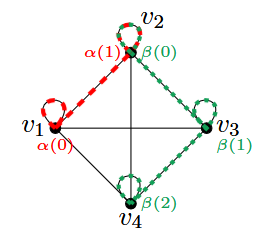
\includegraphics[width=0.3\textwidth]{figures/concatenation-input}
			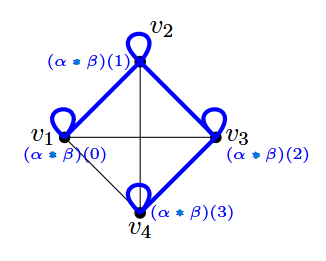
\includegraphics[width=0.35\textwidth]{figures/concatenation-output-bearbeitet}
			\caption{Example of the concatenation of two walks}
			\label{fig:concatenation}
		\end{figure}

	We are finally able to present the notion of $\times$-homotopy.	In the traditional homotopy theory of topological spaces, a homotopy is a continuous map $X\times[0,1]\to Y$, which for ``nice'' spaces can be equivalently thought of as a continuous map $X^{[0,1]}\to Y$. In the discrete setting, this latter description often turns out to be more useful, so we will introduce a $\times$-homotopy in this form. The product-exponential adjunction then allows us to recover the probably more common form as a morphism on the product.
	
	\begin{defi}
		Let $f,g\co G\to H$ be graph morphisms.
		A \textit{$\times$-homotopy of length~$n$ from $f$ to~$g$} is a looped walk in~$H^G$ of length~$n$ from $f$ to~$g$, that is, a graph morphism $\lambda\co I^n_\ell\to H^G$ satisfying $\lambda(0)=f$ and $\lambda(n)=g$.
		We say that $f$ is \textit{$\times$-homotopic} to~$g$ iff there exists such a $\times$-homotopy~$\lambda$.
		In this case, we also write $f\simeq g$ via~$\lambda$.
			%
		Since we will here only deal with $\times$-homotopy, we will henceforth simply speak of \textit{homotopy} and \textit{homotopic}.
	\end{defi}

	It is often convenient to use one of the following equivalent characterizations of homotopies:
		\begin{align*}
			&\{ \textup{homotopies of length } n \textup{ from } f \textup{ to } g \} \\[4pt]
			= &\{ \textup{graph morphisms } \lambda\co I^n_\ell\to H^G \textup{ with } \lambda(0)=f \textup{ and } \lambda(n)=g \} \\[8pt]			
			\cong &\{ \textup{graph morphisms } \Lambda\co G\times I^n_\ell\to H \textup{ with } \Lambda(-,0)=f \textup{ and } \Lambda(-,n)=g \} \\[8pt]
			\cong &\{ \textup{sequences } (f_0,f_1,\dots,f_n) \textup{ of graph morphisms } f_i\co G\to H \textup{ such that } \\
			&\quad f_0=f, f_n=g \textup{ and } \forall i\in\{1,\dots,n\}: f_{i-1}\sim f_i\in E(H^G) \}.
		\end{align*}

	Let us observe that there exists a homotopy of length \textbf{one} from $f$ to~$g$ if and only if $f\sim g\in E(H^G)$.
	
	\begin{rmk}
		Being homotopic defines an equivalence relation on the set $\textup{Gph}(G,H)$ of graph morphisms from $G$ to~$H$.	
	\end{rmk}
		
	\begin{lemma}
		Let $g,g'\co G\to H$ be graph morphisms, and let $\lambda\co I^n_\ell\to H^G$ be a homotopy from $g$ to $g'$.
		\begin{enumerate}
		\renewcommand{\labelenumi}{(\theenumi)}
			\item Every graph morphism $h\co H\to J$ induces a homotopy  
			\[ h_\ast\lambda\co I^n_\ell\to J^G, \quad i\mapsto h\comp\lambda(i) \]
			from $h\comp g$ to $h\comp g'$.
			\begin{equation*}
				\begin{tikzcd}[row sep=small]
					G \arrow[rr, "(h_\ast\lambda)(i)"] \arrow[rd, 	"\lambda(i)", swap] 
					& & H \arrow[ld, "h"] 
					\\ & J
				\end{tikzcd}
			\end{equation*}			

			\item In a similar manner, for every graph morphism $f\co F\to G$,
			\[ f^\ast\lambda\co I^n_\ell\to H^F, \quad i\mapsto \lambda(i)\comp f \]
			is a homotopy from $g\comp f$ to $g'\comp f$.
			\begin{equation*}
				\begin{tikzcd}[row sep=small]
					F \arrow[rr, "f"] \arrow[rd, "\lambda(i)", swap] 
					& & G \arrow[ld, "(f^\ast\lambda)(i)"] 
					\\ & H
				\end{tikzcd}
			\end{equation*}			
		\end{enumerate}
	\end{lemma}

	Let us now explain how homotopies may be composed horizontally.
	For this, let $f,f'\co G\to H$ and $g,g'\co H\to J$ be graph morphisms, and suppose that $f$ is homotopic to~$f'$ via some homotopy $\lambda\co I^n_\ell\to H^G$ and that $g$ is homotopic to~$g'$ via $\gamma\co I^m_\ell\to J^H$.
	Then by above,
		\begin{align*}
			g\comp f\simeq g\comp f' \quad &\textup{via} \quad g_\ast\lambda\co I^n_\ell\to J^G \qquad \textup{and} \\
			g\comp f'\simeq g'\comp f' \quad &\textup{via} \quad f'^\ast\gamma\co I^m_\ell\to J^G.
		\end{align*}
	As a consequence, we have
		\begin{equation*}
			g\comp f\simeq g'\comp f' \quad \textup{via} \quad \lambda\ast\gamma\coloneqq (g_\ast\lambda)\bigcdot(f'^\ast\gamma)\co I^{n+m}_\ell\to J^G.
		\end{equation*}
	Explicitly, for all $i\in\{0,\dots,n+m\}$, the homotopy $\lambda\ast\gamma$ is given at vertex~$i$ by
		\begin{equation*}
			(\lambda\ast\gamma)(i) = \begin{cases}
				g\comp\lambda(i) & i\in\{0,\dots,n\} \\
				\gamma(n-i)\comp f' & i\in\{n,\dots,n+m\}.
			\end{cases}			
		\end{equation*}

	\begin{defi}
		We call $\lambda\ast\gamma = (g_\ast\lambda)\bigcdot(f'^\ast\gamma)$ the \textit{horizontal composition of $\lambda$ and~$\gamma$}.
	\end{defi}

	Note that we also have
		\begin{equation*}
			g\comp f\simeq g'\comp f' \quad \textup{via} \quad \lambda\wt{\ast}\gamma\coloneqq (f^\ast\gamma)\bigcdot(g'_\ast\lambda)\co I^{m+n}\to J^G
		\end{equation*}
		using that
		\begin{align*}
			g\comp f\simeq g'\comp f \quad &\textup{via} \quad f^\ast\gamma\co I^m_\ell\to J^G \qquad \textup{and} \\
			g'\comp f\simeq g'\comp f' \quad &\textup{via} \quad g'_\ast\lambda\co I^n_\ell\to J^G.
		\end{align*}

	\noindent This raises the question whether these two homotopies $\lambda\ast\gamma$ and $\lambda\wt{\ast}\gamma$ are the same. Unfortunately, the answer is ``no''. But: They are homotopic rel endpoints.

	\begin{defi}
		Let $f,g\co G\to H$ be graph morphisms, and let $\lambda,\gamma\co I^n_\ell\to H^G$ be two homotopies from $f$ to~$g$.
		A \textit{homotopy rel endpoints of length $k$ from $\lambda$ to~$\gamma$} is a homotopy $\theta\co I^k_\ell\to (H^G)^{I^n_\ell}$ of length $k$ from $\lambda$ to $\gamma$ which additionally satisfies $\theta(i)(0)=f$ and $\theta(i)(n)=g$ for each $i\in\{0,\dots,k\}$, that is, each $\theta(i)\co I^n_\ell\to H^G$ is a homotopy from $f$ to~$g$.
	\end{defi}

	\begin{prop}
		The two homotopies $\lambda\ast\gamma$, $\lambda\wt{\ast}\gamma\co I^{n+m}_\ell\to J^G$ are homotopic rel endpoints.
	\end{prop}
		
	For $n=m\in\{2,3\}$, an idea of proof is illustrated by the following diagrams:
	\begin{figure}[H]
		\centering
		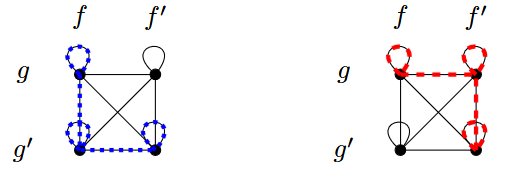
\includegraphics[width=0.6\textwidth]{figures/homotopy-n-m-2}
		\caption*{$\hspace{1cm} (f^\ast\gamma)\bigcdot(g'_\ast\lambda) \hspace{4cm} (g_\ast\lambda)\bigcdot(f'^\ast\gamma)$}
	\end{figure}

	\begin{figure}[H]
		\centering
		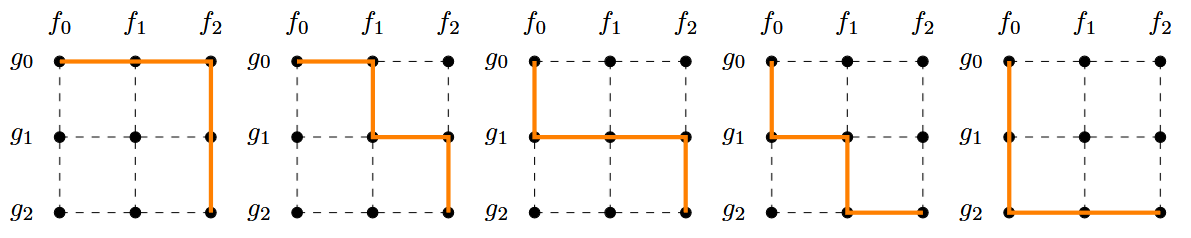
\includegraphics[width=\textwidth]{figures/homotopy-n-m-3}
	\end{figure}

	We endow the 1-category $\Grph$ with the structure of a (strict) 2-category as follows:
	
	\begin{itemize}
		\item The objects are graphs.
		
		\item For any graphs $G$ and $H$, the 1-cells from $G$ to $H$ are the graph morphisms $G\to H$.
		
		\item For any graph morphisms $f,g\co G\to H$, the 2-cells from $f$ to~$g$ are the homotopy rel endpoints classes $[\lambda]$ of homotopies $\lambda$ from $f$ to~$g$ (of any length).
		
		\begin{equation*}
			\begin{tikzcd}[column sep=large]
				G 
				\arrow[bend left=50]{r}{f}
				\arrow[r, phantom, "\Downarrow\mathsmaller{[\lambda]}"]
				\arrow[bend right=50, swap]{r}{g}
				& H
			\end{tikzcd}
		\end{equation*}

		\item The composition of 1-cells $f\co G\to H$ and $g\co H\to J$ is the usual composition of graph morphisms, $g\comp f\co G\to J$.

		\item For any triple of graph morphisms $f,g,h\co G\to H$, the vertical composition of 2-cells $[\lambda]\co f\Rightarrow g$ and $[\gamma]\co g\Rightarrow h$ is defined by concatenation of homotopies: $[\lambda\bigcdot\gamma]\co f\Rightarrow h$.

		\item For any quadruple of graph morphisms $f,f'\co G\to H$ and $g,g'\co H\to J$, the horizontal composition of 2-cells $[\lambda]\co f\Rightarrow f'$ and $[\gamma]\co g\Rightarrow g'$ is defined by horizontal composition of homotopies: $[\lambda\ast\gamma]\co g\comp f\Rightarrow g'\comp f'$.
	\end{itemize}
	
\nocite{*}
\printbibliography


\end{document}